\chapter{Overview} %Last updated 31-1-2016
\label{ch:oversub}

In \Cref{ch:intro} the initial topic was introduced: \acl{MSR} high-thrust ascent trajectory and low-thrust orbiter trajectory combined optimisation. Within this topic it is hypothesised that a rendezvous between the high-thrust \acf{MAV} and the low-thrust Mars 2022 orbiter in less than one revolution after \ac{MAV} launch would benefit both total mission mass and time. This initial topic is based on the proposed \acf{MSR} mission by \ac{JPL}\footnote{\label{foot:jpl_missions} All \ac{JPL} missions: \url{http://www.jpl.nasa.gov/missions/} [Accessed 30 July 2015]} and is interesting because of the many different aspects of this mission. It will involve the integration and optimisation of the ascent trajectory of the \ac{MAV} to low Mars orbit. Once in orbit, the \ac{MAV} will have to rendezvous with an orbiting \ac{s/c}. The current proposal involves the Mars 2022 orbiter, which will use a low-thrust propulsion system to manoeuvre in the Martian system and will initially be used to perform scientific measurements. The orbiter must then perform several orbit changes to position itself in the desired rendezvous orbit. This low-thrust trajectory will have to be integrated and optimised as well. At the start of this literature study it is proposed to combine these two trajectory optimisations in order to find the optimal total mission mass and time. The different aspects of this proposal will be investigated in this literature study to determine the different possibilities for Mars ascent trajectories, low-thrust orbital trajectories,  rendezvous in less than one revolution after launch, integration and optimisation of the trajectories. The final thesis proposal will be based on the information gathered and trade-offs perform in this study.




%\section{Searching for subjects}
%\label{sec:search}
%Since the thesis research is performed at NASA \ac{JPL} under their supervision it made sense to investigate the different missions that they have planned for the near future. An overview is provided on the \ac{JPL} website \footnote{\label{foot:jpl_missions} All \ac{JPL} missions: \url{http://www.jpl.nasa.gov/missions/}}. Two of the future and proposed missions to Mars were \ac{MSR} and Mars 2020. The \ac{MSR} mission is described as a mission that would return samples to Earth using a \ac{MAV} to launch from the Martian surface. The \ac{MAV} would contain rock, soil and atmospheric samples to be analysed back on Earth. The Mars 2020 mission (also sometimes referred to as the Mars Science Laboratory 2 mission) will be the next rover mission to Mars. Its prime goal will be to investigate the (past) habitability of Mars, and assess natural resources and possible hazards to help in the preparation of future human expeditions $^{\ref{foot:jpl_missions}}$. It is in its concept similar to the current Curiosity mission. Provided these two missions, it was then decided to formulate thesis subjects in correspondence with these missions but also correlate to personal preferences. This resulted in six thesis topics which were presented to \ac{JPL} after which the topic selection process was started. Together with the supervisors at the TU Delft and at \ac{JPL} it was decided to work out one of these topics in particular and write it into a proposal. Because the expertise of the section is on orbits it was decided to focus on \ac{MSR}, which also fits well with the current work of the \ac{MPFO} whom are designing the orbits for the Mars 2022 orbiter. The result is an initial thesis proposal that will be described in the next section.
%
%%As can be read in the next section, I was able to combine this into one topic. 
%
%%\section{Initial concepts}
%%\label{sec:inicon}
%%The first subject was based on the \ac{MSR} mission and incorporated the desire to work on both launcher trajectory and orbit optimisation. Therefore this subject was called \textbf{\textit{"Mars Sample Return launch trajectory"}}. 
%%
%%The goal would be to optimise the whole journey of the samples back to Earth starting with a Martian launch, then performing the transfer orbits to get it back to Earth, and finally re-entry to land the samples safely on Earth.\\
%%The second subject was based on the Mars 2020 mission and was mainly focussed on a Martian descent similar to the \ac{MSL} 1. This was interesting because the \ac{MSL} 1 mission had a very interesting descent phase consisting of several stages. The challenge here would be to see if this would be useful for a second mission as well, if so; where could it be improved. If not, what would be a better solution for Mars 2020 instead. This second subject was therefore called \textbf{\textit{"Mars Science Laboratory 2/Mars 2020 descent analysis"}}.\\
%%These were the initial subjects that were used during the early phases of the topic iteration process. This first iteration resulted in three thesis topics per corresponding subject. This was the result of some initial research into the subjects.
%%
%% These six topics were then presented to \ac{JPL} and the topic selection process was started. Together with the supervisors at the TU Delft and at \ac{JPL} it was decided to work out one of these topics in particular and write it into a proposal. Because the expertise of the section is on orbits it made more sense to go for \ac{MSR}, and this also fit well with the \ac{MPFO} since they want to design the orbits for the Mars 2022 orbiter. As can be read in the next section, I was able to combine this into one topic. 
%
%\section{Initial proposal}
%\label{sec:curprop}
%In this section the initial (starting) proposal is discussed based on the different aspects of a proposal as taught by the course Research Methodologies at the TU Delft. The initial working title is \textbf{\textit{"\acl{MSR} precise point rendezvous in Mars orbit}}. Please note that this is not the final proposal and will change due to the knowledge gained and provided in this literature study. 
%
%\subsection{Research objective}
%\label{subsec:resobj}
%The objective of this research is to find the optimum combination of the high-thrust \ac{MAV} launch trajectory and the orbital changes required for the low-thrust orbiter to rendezvous at a certain point above Mars, depending on the desired design choices, and returning the orbiter to a safe orbit by using \ac{TSI} to propagate the trajectories, Q-law to determine the low-thrust orbiter thrust curve and using \ac{DE} combined with and compared to \ac{MBH} to optimise for mass, \ac{ToF}, $\Delta V$,  $I_{sp}$ and/or $\theta$. 
%
%
%%\nomenclature{$ToF$}{Time of Flight\nomunit{s or days}}
%
%\subsection{Research perspective}
%\label{subsec:respers}
%It will be both Theory-testing research (\ac{TSI}, \ac{DE} and \ac{MBH}) and Problem-analysis research (optimum problem). The problem will be solved through the writing and validation of an optimisation program based on orbital mechanics and from a(n) (initial) mission design standpoint. It is therefore an engineering problem, and is a result of preliminary research and discussions between researchers, supervisors and stakeholders. 
%
%\subsection{Research framework}
%\label{subsec:resfram}
%The framework has been set-up based on the guidelines provided in Research Methodologies and the corresponding literature \cite{verschuren2010design} and is visualized in \Cref{fig:resframe}.
%
%\begin{figure}[!ht]
%\centering
%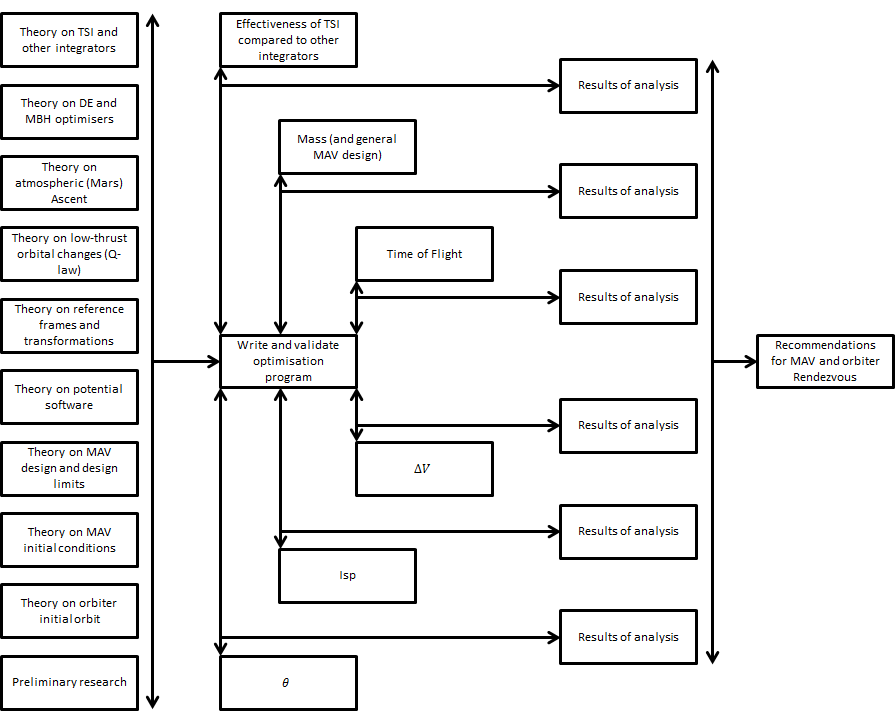
\includegraphics[width=0.9\textwidth]{figures/overview/resframe.png}
%\caption{Research framework for the literature study (a) and the thesis work (b, c \& d)}
%\label{fig:resframe}
%\end{figure}
%
%\textit{Formulation:} (a) the study of the different theories and the preliminary research will result in a model (b) that can be used to write and validate an optimisation program to optimise for the different parameters and also determine the usefulness of \ac{TSI}. (c) A comparison of the different optimisation results will help (d) establish the recommendations for the optimum \ac{MAV} and orbiter rendezvous above Mars.
%
%\subsection{Research questions}
%\label{subsec:resques}
%The corresponding research questions are listed:\\
%
%
%%\begin{easylist}
%%\ListProperties(Hide=100, Hang=true, Progressive=3ex, Style*=--,Style2*=$\circ$)
%%& What are the current integration and optimisation methods used to perform ascent and transfer trajectory optimisation, how are the proposed methods different, and what are the expected results?
%%&& What is the difference between \ac{TSI} and other frequently used integration methods in ascent and transfer trajectory calculations/optimisation and how do they work?
%%&& Which different optimisation methods are used in ascent and transfer trajectory optimisation and why have \ac{DE} and \ac{MBH} been chosen?
%%\end{easylist}
%
%\begin{itemize}
%\item What are the current integration and optimisation methods used to perform ascent and transfer trajectory optimisation, how are the proposed methods different, and what are the expected results?
%\begin{itemize}
%\item What is the difference between \ac{TSI} and other frequently used integration methods in ascent and transfer trajectory calculations/optimisation and how do they work?
%\item Which different optimisation methods are used in ascent and transfer trajectory optimisation and why have \ac{DE} and \ac{MBH} been chosen?
%\item What is the difference between \ac{DE} and \ac{MBH}, how do they work and what are the expected results?
%\item Which integration method(s) will \ac{TSI} be compared to, why these particular integration methods and what are the expected improvements of \ac{TSI} with respect to the other methods?
%\end{itemize}
%\item Which aspects, parameters and equations are involved when designing ascent and transfer trajectories, what is the underlying theory and how can it be applied here?
%\begin{itemize}
%\item What are the different aspects, parameters and equations when simulating an atmospheric ascent and how does that translate to Mars?
%\item How can a low-thrust orbit transfer be performed and optimised for a rendezvous in Mars orbit?
%\item Which perturbing bodies have to be accounted for in the Mars system to provide an accurate representation and which other perturbing sources have to be taken into account?
%\item Which frame(s) of reference will need to be used, and if more than one frame is required, how do they relate to each other?
%\item What will be the starting conditions of the \ac{MAV} and the orbiter?
%\item How do the different parameters affect the design of the \ac{MAV}, how much can it be changed and what are the design limits, and thus also parameter limits, for the \ac{MAV}?
%\item When aiming for an orbit using Q-law, how can a precise orbit position be incorporated?
%\end{itemize}
%\item What are the different optimal rendezvous situations given different design choices?
%\begin{itemize}
%\item How does the orbit of the orbiter have to change to reach the desired rendezvous point based on the design choices?
%\item What is the best \ac{MAV} configuration and combination of launch parameters to reach the desired rendezvous point based on the design choices?
%\item Which design is optimal for which design choice(s)?
%\end{itemize}
%\item Would \ac{TSI} be a good alternative for use in future optimisation programs?
%\begin{itemize}
%\item How much more (or less) accurate is \ac{TSI} compared to the other chosen integration methods?
%\item How much faster (or slower) is \ac{TSI} compared to the other chosen integration methods?
%\item What are the advantages and disadvantages (besides the first two sub-questions) when using \ac{TSI} in this kind of trajectory optimisation problem?
%\end{itemize}
%\item Which of the two (or what kind of combination of the two) optimisation methods worked best in this kind of trajectory optimisation problem, what are the advantages and disadvantages of the different methods? 
%\end{itemize}
%
%\subsection{Research strategy}
%\label{subsec:resstrat}
%The first step will be to perform a literature study on the subject, collect all the theory and become acquainted with this theory. The \ac{TSI} should be explained in detail as well as the chosen reference integration method. The same will have to be done for \ac{DE} and \ac{MBH} as well as the Q-law method. After completion of the literature study, the optimisation program will have to be written, using the \acl{TSI}, to optimise (utilizing both \ac{DE} and \ac{MBH}) Martian ascent to a certain parking/rendezvous orbit starting at different elevations, azimuth and launch angle with respect to the horizon. This would also be used to compare the \acl{TSI} with one (or a number of) other integration method(s), for a small number of orbits, to identify the most suitable integrator for this problem. Once this is completed, the program should be updated such that this ascent optimisation will be able to not just optimise to a certain parking/rendezvous orbit but to also get to a specific point in that orbit (include time and $\theta$) to perform a rendezvous manoeuvre with the orbiter. For the \ac{MAV} this means that it could either directly go to the rendezvous point or first into a parking orbit (starting on the Martian surface) and then to the rendezvous orbit and point. It is assumed that during the entire ascent and manoeuvring phase the \ac{MAV} uses a high-thrust propulsion system. As soon as this part of the program is validated, the orbiter can be added as well including Q-law. Given that the orbiter, which uses a low-thrust propulsion system, starts from a scientific orbit, optimise the rendezvous orbit and point such that both \ac{MAV} and orbiter will be at that point at the same time. After which the orbiter will have to go back to a higher orbit to avoid getting caught in the gravity well of Mars. During each stage of the program writing it will have to be verified and validated. The validation will be performed based on the results from current \ac{JPL} software used to perform orbit trajectory analyses and reference data from flown missions. Once the program validation has been completed, the actual optimisation process can commence and the optimisation will be performed for a number of different design choices while keeping within the limits of the \ac{MAV} design and the orbiter design. Finally, recommendations will be provided based on the different optimised results and design choices.
%
%\subsection{Research Method}
%\label{subsec:resmeth}
%The research will be performed using a self-written software program and validated with flight data and results from simulations performed with programs used by \ac{JPL}.